\section{Zielsetzung}
\label{sec:Zielsetzung}
Dieser Versuch beschäftigt sich mit dem Michelson-Interferometer.
Mit dessen Hilfe wird zuerst die Wellenlänge eines Lasers ausgemessen.
Anschließen wird noch der Brechnungsindex von Luft ermittelt.


\section{Theorie}
\label{sec:Theorie}

\subsection{Interferenz und Kohärenz von Licht}

Da im Interferometer Interferenzeffekte auftreten, werden im folgenden Abschnitt die Voraussetzung für Interferenz vorgestellt.
Licht wird in diesem Fall als elektromagnetische Welle betrachtet, sodass seine Ausbreitung mit den Maxwellgleichungen beschrieben werden können. Die Beschreibung der 
Lichtwelle erfolgt über
\begin{equation}\label{eqn:licht}
    \vec{E}(x,t) = \vec{E_0} \cos(kx-wt-\delta),
\end{equation}
wobei $k$ die Wellenzahl ist, welche über $k=\frac{2\cdot \pi}{\lambda}$ im Zusammenhang mit der Wellenlänge $\lambda$ steht, $\omega$ die Kreisfrequenz, und 
$\delta$ der Phasenwinkel ist. Die messbare Größe ist aber die Intensität $I$ des Lichtes, welche über $I = |\vec{E}|^2$  berechnet wird. Sie beschreibt den Zeitmittelwert der
Lichtleistung, die auf eine Flächeneinheit trifft. \\
Treffen zwei Lichtwellen auf einen Punkt auf, überlagern sie sich nach dem Superpostionsprinzip. Daher folgt für die Intensität:
\begin{equation*}
    I_{\text{ges}} = \frac{1}{t_2 - t_1} \int_{t_1}^{t_2} | \vec{E}(x,t)|^2 \, \symup{d}t  = \frac{1}{t_2 - t_1} \int_{t_1}^{t_2} | \vec{E_1}+ \vec{E_2}|^2 (x,t) \, \symup{d}t
\end{equation*}
Hierbei sollte der Beobachtungszeitraum groß gegenüber der Periodendauer sein. 
Werden nun beide der Lichtwellen mit Funktionen der Form \eqref{eqn:licht} beschrieben, dann ergibt sich für die Gesamtintensität der Wert $I_{\text{ges}} = 2 \vec{E_0}^2 (1+\cos(\delta_2 - \delta_1))$.
Der sogenannte Interferenzterm $2\vec{E_0}^2 \cos(\delta_2 - \delta_1)$ zeigt, dass sich die einzelnen Intensitäten der Lichtwellen nicht einfach addieren.\\

\noindent
Interferenz tritt nicht bei jedem Licht auf; um Interferenzeffekte zu beobachten, wird kohärentes Licht benötigt. Das bedeutet, dass sich das Licht durch eine Funktion der Form \eqref{eqn:licht}
darstellen lässt, wobei die Parameter $k$, $\omega$ und $\delta$ einen festen Wert haben. Laser erzeugen kohärentes Licht, jedoch ist auch mit normalen Lichtquellen kohärentes Licht
erzeugbar. Hierfür wird, wie in der \autoref{fig:wegunterschied} zu sehen ist, das Licht aus einer Lichtquelle durch eine Doppelblende aufgeteilt und über Spiegel auf einen Schirm
gelenkt. 

\begin{figure}
    \centering
    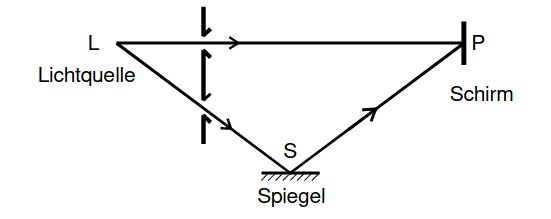
\includegraphics[width=0.5\textwidth]{content/wegunterschied.jpg}
    \caption{Versuchsanordnung zur Erzeugung von kohärentem Licht aus einer konventionellen Lichtquelle \cite{anleitung}.}
    \label{fig:wegunterschied}
\end{figure}

\noindent
Jedoch ist zu beachten, dass der Emissionsakt nur eine endliche Zeit $\tau$ währt, also der emittierte Wellenzug eine endliche Länge. Ist der Wegunterschied $\increment $ (in \autoref{fig:wegunterschied}
$\increment = \overline{\text{LSP}} - \overline{\text{LP}} $ ) deutlich größer als die Länge des Wellenzuges, treten keine Interferenzeffekte auf. Dies kommt daher, dass die Lichtwellen,
welche dann zeitgleich an dem Punkt P ankommen, keine feste Phasenbeziehung mehr haben, also nicht mehr kohärent sind. Der Wegunterschied, bei dem gerade keine Interferenzeffekte mehr 
beobachtet werden, wird Kohärenzlänge genannt.\\
Nach dem Fourierschem Theorem kann ein Wellenzug endlicher Länge nicht monochromatisch sein, jedoch ist polychromatisch oder nicht-monochromatisches Licht im allgemeinen nicht 
interferenzfähig. Daher muss darauf geachtet werden, dass das Frequenzspektrum so schmal oder der Wegunterschied klein genug ist, sodass die Maximums- und Minimumsbedingungen von zwei
Wellenlängen nicht an demselben Ort realisiert werden können.


\subsection{Prinzipieller Aufbau des Michelson-Interferometers}

Das Michelson-Interferometer wurde entwickelt um im Michelson-Morley-Experiment den Äther nachzuweisen, welches nicht funktiomiert hat, jedoch werden ähnliche Interferometer benutzt
um Gravitationswellen nachzuweisen. Der prinzipielle Aufbau des Michelson-Interferometers ist in \autoref{fig:prinzipmichelson} zu sehen. In dem Punkt L ist die Lichtquelle stationiert,
welche das Licht auf eine semipermeable Platte P emittiert. Dort wird der Lichtstrahl aufgespalten. Der reflektierte Strahl wird auf die Strecke zum Spiegel $\symup{S_1}$ geschickt, 
an dem Spiegel wird das Licht komplett reflektiert. Der transmittierte Strahl läuft auf den Spiegel $\symup{S_2}$ zu und wird dort reflektiert. Beide Strahlen treffen wieder auf den
semipermeablen Spiegel, der vorher transmittierte Strahl wird reflektiert und der vorher reflektierte Strahl wird transmittiert, sodass beide Strahlen auf dem Weg zum Detektor D sind.
Damit die einzelnen Strahlen beim Wiederaufeinandertreffen am semipermeablen Spiegel P interferenzfähig sind, darf der Weglängenunterschied 
$ \increment = 2\overline{\text{PS}_2} - 2\overline{\text{PS}_1} $ nicht länger als die Kohärenzlänge sein. Die Kompensationsplatte in der Strecke
$\overline{\text{PS}_2}$  hat den gleichen Brechungsindex wie der semipermeable Spiegel; somit wird ausgeglichen, dass der reflektierte Strahl dreimal,
während der transmittierte Strahl nur einmal durch P geht.
\begin{figure}
    \centering
    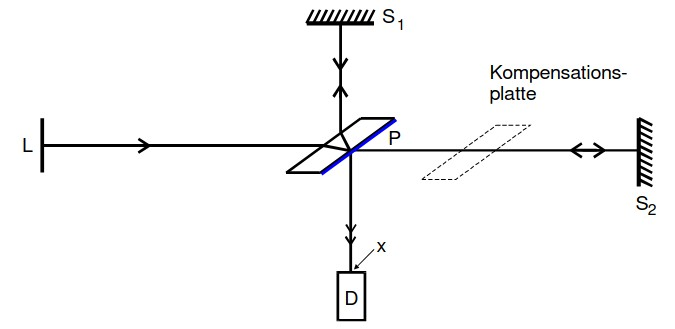
\includegraphics[width=0.5\textwidth]{content/prinzipmichelson.jpg}
    \caption{Der schematische Aufbau des Michelson-Interferometers \cite{anleitung}.}
    \label{fig:prinzipmichelson}
\end{figure}

\noindent
Sind die Strecken $\overline{\text{PS}_1}$ und $\overline{\text{PS}_2}$ gleich lang, haben die Lichtstrahlen am Detektor D einen Gangunterschied von $\frac{\lambda}{2}$, sodass 
destruktive Interferenz auftritt und sich die Strahlen auslöschen, es wird keine Intensität gemessen. Wird nun einer der Spiegel um die Strecke $\increment d$ bewegt, ändert sich
das Interferenzbild. Es gilt die Formel
\begin{equation}\label{eqn:forlambda}
    \increment d = z \cdot \frac{\lambda}{2}, 
\end{equation}
wobei $z$ die Anzahl der beobachteten Interferenzmaxima beschreibt.

\noindent
Außerdem kann in dem Michelson-Interferometer ein optischer Weglängenunterschied aufgebaut werden, in dem, wie in \autoref{fig:brechungsindexaufbau} zu sehen ist, in eine der Strecken
ein Medium mit einem anderen Brechungsindex eingebaut ist.
\begin{figure}
    \centering
    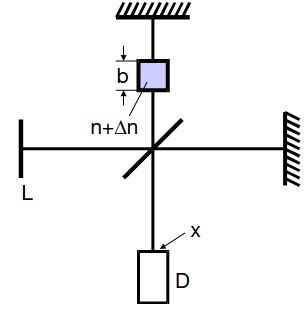
\includegraphics[width=0.25\textwidth]{content/brechungsindexaufbau.jpg}
    \caption{Der prinzipielle Versuchsaufbau zur Messung von Brechungsindices mit Hilfe des Michelson-Interferometers \cite{anleitung}.}
    \label{fig:brechungsindexaufbau}
\end{figure}
\noindent
Der Weglängenunterschied der beiden Strahlen beträgt hier $\increment = \increment n \cdot b$. Bei der Änderung von dem Druck in der Kammer, lassen sich $z$ Maxima beobachten. Es gilt
\begin{equation*}
    \increment n \cdot b = z \cdot \frac{\lambda}{2}
\end{equation*}
Beschreibt $N$ die Anzahl der Dipole pro Volumeneinheit, die von der Lichtwelle zu Schwingungen erzwungen wurden, so kann aus der klassischen Dispersionstheorie 
\begin{equation*}
    n = \sqrt{1+ f(\lambda)N}
\end{equation*}
gefolgert werden. Da die hier zu untersuchende Gase im Bereich von 0 bis $\SI{1}{\bar}$ sich wie ideale Gase verhalten, kann die Ideale Gasgleichung benutzt werden, 
sodass gilt:
\begin{equation*}
    N(r,T) = \frac{p}{T}\frac{T_0}{p_0} N_{\text{L}}
\end{equation*}
Der Unterschied des Brechungsindex des Gases zu dem der Umgebung lässt sich angeben durch $\increment n(p, p') = \frac{f}{2} ( N(p,T) - N(p',T) )$. Soll der 
Brechungsindex unter Normalbedingungen angegeben werden, so ergibt sich die Formel zu:
\begin{equation*}
    n(p_0, T_0) = 1 + \increment n(p, p') \frac{T}{T_0} \frac{p_0}{p - p'}
\end{equation*}
Somit kann der Brechungindex des Gases schließlich über
\begin{equation}\label{eqn:forindex}
    n = 1 + z \cdot \frac{\lambda}{2b} \cdot \frac{T}{T_0} \frac{p_0}{p - p'}
\end{equation}
errechnet werden.